\documentclass[sigconf]{acmart}

\usepackage{hyperref}

\usepackage{subfig}

\usepackage{listings}
\lstset{
  columns=fullflexible, 
  frame=single,
  breaklines=true,
}

\AtBeginDocument{
  \providecommand\BibTeX{{
    \normalfont B\kern-0.5em{\scshape i\kern-0.25em b}\kern-0.8em\TeX}}}

\setcopyright{none}
\copyrightyear{}
\acmDOI{}
\acmISBN{}
\acmConference[Data Science Seminar]{Data Science Seminar}{2019}{Uni Passau}


\begin{document}

\title{[Experiment] Learning Community Embedding with Community Detection and Node Embedding on Graph (CD)}

\author{Anton Begehr}
\affiliation{
  \institution{University of Passau}
  \streetaddress{Innstraße 33}
  \city{Passau}
  \country{Germany}}
\email{a.begehr@fu-berlin.de}


\begin{abstract}
  The graph embedding algorithm ComE developed by \citeauthor{Cav17} in their \citeyear{Cav17} paper \textit{Learning Community Embedding with Community Detection and Node Embedding on Graph} combines the powers of community detection, community embedding, and node embedding in a closed loop optimizing algorithm to generate low dimensional embeddings for communities and nodes in a graph. This research paper undertakes an experiment with the aims to explore ComE's inner workings and measure its effectivity of classifying crawled Twitter data in comparison to Louvain Modularity with normalized mutual information.
\end{abstract}


\maketitle

\begin{figure}
    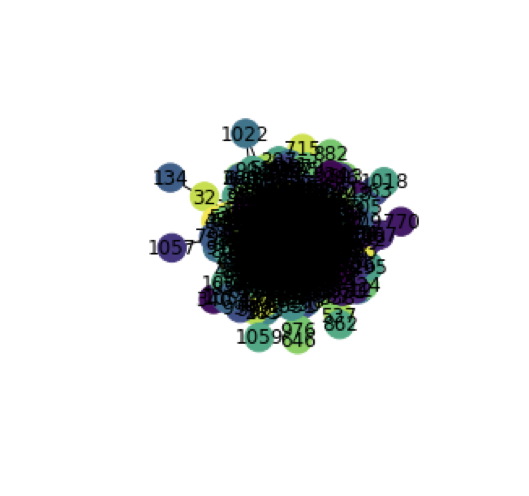
\includegraphics[width=\linewidth]{graphics/graph_ComE.png}
    \caption{\textit{arthrocon} graph plotted by ComE}
    \label{graph_ComE}
\end{figure} 

\section{Introduction}

In their \citeyear{Cav17} paper \textit{Learning Community Embedding with Community Detection and Node Embedding on Graph} the authors \citeauthor{Cav17} explore graph embeddings by utilizing a three step closed loop optimization process consisting of Community Detection, Community Embedding, and Node Embedding: ComE.\cite{Cav17} They then apply ComE and further graph embedding algorithms on excerpts of multiple, well known graph datasets: Karate Club, BlogCatalog, Flicker, Wikipedia, DBLP. They choose DeepWalk/SF, Line, Node2Vec, GraRep, and M-NMF to measure the quality of ComE's results using Micro-F1 and Macro-F1 for classification results and conductance and normalized mutual information (NMI) for the resulting graph embeddings. It is worthwhile to note, that ComE works with elementary graphs, meaning graphs consisting of nodes and edges, disregarding, for example, node properties, edge properties, and edge weights.

In this paper we will explore the graph embedding algorithm ComE developed by \citeauthor{Cav17}, generate embeddings using ComE for the Twitter dataset \cite{TwitterData} crawled by \citeauthor{TwitterData}, and compare the results to communities gained by applying Louvain Modularity using normalized mutual information (NMI) as a comparison measure.


\section{Twitter Data} \label{Twitter_data}

Crawled datasets from Twitter, combined with conference data that is supplied in the public GitHub repository \textit{fatemehsrz/Twitter\_Data} will be used.\cite{TwitterData}

\subsection{Exploration}

The supplied Twitter data consists of three groups. Each concerning the Twitter interactions of a user either attending or not attending one of three conferences. The three conferences are labeled as (1) \textit{anthrocon}, (2) \textit{comiccon2017}, and (3) \textit{icann2016}.

For each conference two CSVs are supplied:

\begin{enumerate}
	\item tweets: For each tweet an unique identifier, the content of tweet, an identifier for the user who posted the tweet and a label determining if the suer attended the conference is supplied. 
	\item edgelist: Each row represents an edge between two users. It will be assumed, that each edge represents an interaction on Twitter. For example commenting and liking would count as interactions.
\end{enumerate}

The tweets id and content will be disregarded in our investigation, because we assume the tweet id does not include information we can utilize since ComE does not support property graphs and we will not be participating in any NLP practices in this experiment.

The tweet and edges datasets of the conferences have the following metrics:

\begin{enumerate}
	\item \textit{anthrocon}
	\begin{itemize}
		\item tweets: $3842$
		\item users: $1060$
		\item edges: $15788$
		\item average edges per user: $\approx14.9$
	\end{itemize}
	\item \textit{comiccon2017}
	\begin{itemize}
		\item tweets: $4381$
		\item users: $2495$
		\item edges: $8203$
		\item average edges per user: $\approx3.3$
	\end{itemize}
	\item \textit{icann2016}
	\begin{itemize}
		\item tweets: $2550$
		\item users: $1016$
		\item edges: $17045$
		\item average edges per user: $\approx16.8$
	\end{itemize}
\end{enumerate}

Find the jupyter notebook used for these calculations at \textit{preprocessing/exploratory.ipynb}.

\subsection{Requirements}

Both the problem space and ComE itself have requirements that the data needs to fulfill. The problem space of graph embeddings is first and foremost classification.

Next to obvious requirements of graph embedding algorithms, the following requirements need to be fulfilled to apply ComE on the provided Twitter data specifically:

\begin{enumerate}
	\item The ComE algorithm requires the graph data to be supplied as a \textbf{sparse adjacency matrix}. The example code uses a MATLAB .mat file import. The data supplied by \citeauthor{TwitterData} is in an edge list format inside a CSV file. Each row represents an edge from one node to the other.
	\item ComE requires the nodes to be \textbf{labeled} for training to determine the number K of clusters it should optimize for, also we will be using the ground truth to test the resulting clusters against.
\end{enumerate}

\subsection{Data Preparation}

The two requirements of formatting the graph as a sparse adjacency matrix and the nodes with labels that make sense from an application standpoint will be fulfilled with data preprocessing in the existing ComE infrastructure and outside of it utilizing Jupyter Notebooks. These steps are needed to be able to effectively apply the ComE algorithm on the Twitter data for community embeddings.

\subsubsection{Sparse Adjacency Matrix}
ComE takes a sparse adjacency matrix as input for representing the graph on which to apply the algorithm.

The ComE repository includes functionality in \textit{graph\_utils.py} for importing the graph as a sparse adjacency matrix from a MatLib file.\cite{ComE} The graph obtained from crawling Twitter data is in the format of an edge list with one edge per row of the csv file. To convert an edge list to a sparse adjacency matrix, two functions were added to \textit{graph\_utils.py}:

\begin{itemize}
	\item $adjacency\_matrix\_from\_edges()$
	\item $load\_csv\_edges()$
\end{itemize}

\subsubsection{Labels} ComE requires a labeled training dataset to be able to execute community embeddings. Specifically, ComE determines the number of clusters $K$ from the labels \cite{ComE} and we will be using the ground truth supplied by the labels to test ComE's resulting communities against.

Jupyter notebooks have been chosen for this task, due to the ability to swiftly iterate on solutions and algorithms, also the size of the supplied data allows for local computation on a personal computer.

The preprocessing procedure for the Twitter data mentioned above allows us to utilize ComE's ability to cluster nodes purely from interaction data and then test the results against our ground truth. The ground truth being if a specific user attended an conference or not.

\subsection{Labels}

The users of each conference dataset correspond to the nodes of the graph. Considering we have three datasets with a user identification column, this raises the following question: Do user identifiers apply across conferences? This question is important to know if the conference datasets can be unioned and create an analysis on the whole dataset instead of doing multiple separate analyses.

If the user identifier applies over all three conferences, the data can be unioned and eight labels (communities) could be extrapolated:

\begin{enumerate}
	\item attended no conferences
	\item attended anthrocon
	\item attended comiccon2017
	\item attended icann2016
	\item attended anthrocon, and comiccon2017
	\item attended anthrocon, and icann2016
	\item attended comiccon2017, and icann2016
	\item attended anthrocon, comiccon2017, and icann2016
\end{enumerate}

These eight labels combining the data of all three conferences seemed logical at first and was implemented in the jupyter notebook at \textit{preprocessing/generate\_labels-old.ipynb}.

Further data exploration led to the insight, that the user identifiers for all datasets start with the value $0$ and all user identifiers between the value $0$ and the maximum of the user identifiers for that conference are present in the specific conference. See \textit{preprocessing/user\_ids.ipynb} for detailed insights. Both insights suggest, that the user identifier does not after all apply across conference datasets. Therefore, the conference datasets will need to be tested individually. For each dataset there will be a separate binary labeling:

\begin{enumerate}
	\item did attended conference
	\item did not attended conference
\end{enumerate}

The implementation for binary label generation can be found here: \textit{preprocessing/generate\_labels.ipynb}

\section{ComE}

ComE stands for \underline{Com}munity \underline{E}mbedding. A community is a group of nodes that relate to each other through some concept. A community embedding is a vector representation of such a community.

Most solutions in the space of community embeddings do community detection and node embeddings separately and then aggregate the node embeddings for each detected community to create community embeddings. ComE takes a different, closed-loop, iterable approach. Instead of doing node embeddings and community detection separately, \citeauthor{Cav17} realized that community detection can benefit from node embedding, node embedding can benefit from community embedding, and community embedding in turn benefits from community detection.\cite{Cav17} This creates a closed loop that can be iterated on.

ComE defines community embedding as a multivariate Gaussian distribution. The sum of all community embeddings are a Gaussian mixture model. This allows \citeauthor{Cav17} to do community detection and embedding together in a single objective function based on GMM.\cite{Cav17} Considering each node embedding to be generated by a multivariate Gaussian distribution from a community allows \citeauthor{Cav17} to formulate one likelihood. Given nodes assignments to communities and community embeddings, ComE extends the neural networks of LINE and DeepWalk to preserve first-, second-, and higher-order proximity together and ultimately closes the loop by generating node embeddings through extending the node embedding algorithms LINE and DeepWalk.\cite{Cav17}

\section{Experiment}

The experiment was run on the Twitter data described in Section \ref{Twitter_data} using Python 3.6 and PyCharm 2019.1.4 (Professional Edition). All code that has been used and is written to run this experiment is available at the GitHub repository \textit{abegehr/ASDS\_ComE}:\\\url{https://github.com/abegehr/ASDS_ComE}.\cite{asds}

\subsection{Hyperparameters}

ComE requires setting multiple hyperparameters. Starting with the number $K$ of communities to be identified, over the size of batches to be used for computation, through to the number of iterations the algorithm should run through, many hyperparameters need to be set.
The experiment uses the following hyperparameters:\cite{Cav17}

\begin{lstlisting}[language=python]
# hyperparameters
number_walks = 10  # random walks for each node in sampling
walk_length = 80  # length of each random walk path in sampling
representation_size = 2  # dimensions of embedding space
num_workers = 10  # threads to use for computation
num_iter = 3  # overall iterations to run
reg_covar = 0.00001  # regularization coefficient to ensure positive covariance
batch_size = 50
window_size = 10  # windows size used to compute the context embedding
negative = 5  # number of negative samples
lr = 0.025  # learning rate
alpha_betas = [(0.1, 0.1)]  # array of combinations of alpha and beta
#alpha: Trade-off parameter for context embedding
#beta: Trade-off parameter for community embedding
down_sampling = 0.0
ks = [2]  # array of number of communities
\end{lstlisting}

The hyperparameters have been adjusted to follow advice from the original paper by \citet{Cav17}. Further hyperparameter tuning has not been applied.

\subsection{Process}

The code provided at the GitHub repository \textit{abegehr/ASDS\_ComE}\cite{asds}, which includes the ComE algorithm from the GitHub repository \textit{andompesta/ComE}\cite{ComE} comes in a state where it is ready to run and results are included in the committed data.

If the input data should be altered to run the experiments on a different datasets, running the experiment requires the following steps:

\begin{enumerate}
	\item Generate labels for nodes using the Jupyter notebook \textit{preprocessing/generate\_labels.ipynb} and move to \textit{ComE/data/twitter/twitter.lables}.
	\item Copy edge list to \textit{ComE/data/twitter/twitter.csv}
	\item Open \textit{ComE/} in PyCharm. The input and output file paths in \textit{main.py} should be set correctly.
	\item Run using the BICE configuration with Python 3.6.
	\item This will generate multiple files in \textit{data/}. These are the results of the community embedding.
\end{enumerate}

It is also possible to run ComE a different set of graph data. To accomplish this, the edge list and labeled nodes dataset needs to be placed in the correctly named folder inside \textit{ComE/} and the settings and hyperparameters in \textit{ComeE/main.py} should be configured accordingly. See the original paper by \citeauthor{Cav17}\cite{Cav17} and the associated GitHub repository \textit{andompesta/ComE}\cite{ComE} for further details.

\subsection{Results} \label{apply_ComE}

Running the experiment generates multiple files in \textit{ComE/data/}. The following files are generated:
\begin{itemize}
	\item \textit{twitter\_pre-training.bin}
	\item \textit{twitter/Twitter.walks.*}
	\item \textit{g\_mixture.joblib}: community embedding in the form of a saved binary of the gaussian mixture model where each gaussian represents one community.
	\item \textit{labels\_pred.txt}: predicted labels for each node in the order or nodes supplied by \textit{Twitter.labels}.
	\item \textit{twitter\_alpha-0.1\_beta-5\_ws-10\_neg-5\_lr-0.025\_icom-62\_ind-62\_k-2\_ds-0.0.txt}: node embeddings for each node where each line holds the node id and one value for each of the $K$ dimension of the embedding space.
\end{itemize}

\textit{g\_mixture.joblib}, \textit{labels\_pred.txt}, and \textit{Twitter\_alpha-0.1\_beta-5\_ws-10\_neg-5\_lr-0.025\_icom-62\_ind-62\_k-2\_ds-0.0.txt} can be considered the final results of the algorithm.

ComE was executed for all three conferences: (1) \textit{anthrocon}, (2) \textit{comiccon2017}, and (3) \textit{icann2016}. The resulting files can be found in the GitHub repository \textit{abegehr/ASDS\_ComE}\cite{asds} at:
\begin{enumerate}
	\item anthrocon: \textit{results/data/anthrocon/}
	\item comiccon2017: \textit{results/data/comiccon2017/}
	\item icann2016: \textit{results/data/icann2016/}
\end{enumerate}

To compare the effectiveness of ComE with a proven solutions for community detection on graphs, normalized mutual information (NMI) has been chosen. The normalized mutual information scores for all three conference datasets are as follows:

\begin{enumerate}
	\item \textit{anthrocon}: $NMI_c \approx 0.0007$
	\item \textit{comiccon2017}: $NMI_c \approx 0.0010$
	\item \textit{icann2016}: $NMI_c \approx 0.0031$
\end{enumerate}

These are very low values for normalized mutual information. NMI is defined between $0.0$ and $1.0$, where $1.0$ represents perfect, complete labeling of the data. ComE's NMI scores will be compared with NMI scores obtained by applying Louvain Modularity on the same conference datasets.

\subsection{Louvain Modularity} \label{apply_lm}

Louvain Modularity is an established method for community detection on large networks. It can be used to generate prediction labels from a graph's edges and is less complex in comparison to ComE. To apply Louvain Modularity the number of communities $K$ does not need to be known.

Applying Louvain Modularity on the three conference datasets results in a list of predicted label, one for each node. These labels have been computed in \textit{results/louvain\_modularity.ipynb}. Also normalized mutual information scores have been computed for the labels found by applying Louvain Modularity. The NMI scores obtained through the application of Louvain Modularity are listed here:

\begin{enumerate}
	\item \textit{anthrocon}: $NMI_l \approx 0.0100$
	\item \textit{comiccon2017}: $NMI_l \approx 0.0181$
	\item \textit{icann2016}: $NMI_l \approx 0.0225$
\end{enumerate}

These NMI scores look very similar to the NMI scores obtained by ComE and are very low. Indeed comparable to the NMI scores obtained by ComE.

\subsection{Interpretation}

Both the normalized mutual information scores obtained by applying ComE (section \ref{apply_ComE}) and the NMI scores obtained by applying Louvain Modularity (section \ref{apply_lm}) are very low and represent an insignificant inference of conference attendance from the graph data.

To find out why neither ComE nor Louvain Modularity were able to identify conference attendance from user interactions on Twitter, we can look at one of the conferences in detail. Let's examine the \textit{anthrocon} conference further.

ComE includes a graph utility that provides functionality to plot a graph. The \textit{arthrocon} graph plotted by ComE can be viewed in figure \ref{graph_ComE}. Figure \ref{graph_ComE} shows a tightly packed graph with most nodes tightly connected and a handful of nodes with low connections.

\begin{figure}[H]
    \subfloat[true]{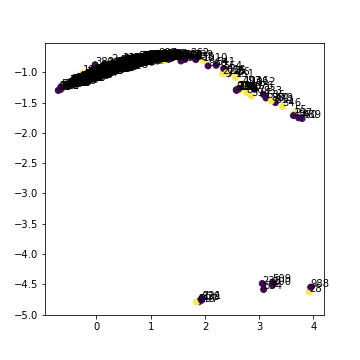
\includegraphics[width=4cm]{graphics/embedding_true_labels.png}}
    \subfloat[predicted]{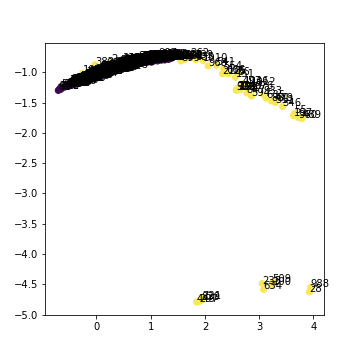
\includegraphics[width=4cm]{graphics/embedding_predicted_labels.png}}
    \caption{\textit{anthrocon} node embeddings colored by labels}
    \label{node_embeddings}
\end{figure}

Figure \ref{node_embeddings} shows two scatter plots which display the node embeddings colored with ground truth labels on the left and predicted labels on the right. The structure of the two dimensional embedding does show a similar setup as the graph in that most nodes are highly interconnected and a handful of nodes are separated.

\textit{Anthrocon} graph and node embedding graphics suggest that the high interconnectivity of the Twitter interaction data provides for increased difficulty of determining the conference attendance. It is possible that the Twitter data does not encompass enough knowledge about the conferences to indicate which users attended the conference and which did not.

The graphs and embeddings resulting from the \textit{comiccon2017} and  \textit{icann2016} datasets look similar to the graph and embedding of the \textit{anthrocon} dataset.

\section{Conclusion}

In this research paper, we have run an experimentation on data crawled from Twitter with the graph embedding algorithm ComE developed by \citeauthor{Cav17} in their \citeyear{Cav17} paper \textit{Learning Community Embedding with Community Detection and Node Embedding on Graph}. ComE's authors claims to combine the powers of community detection, community embedding, and node embedding in a closed loop optimizing algorithm to generate low dimensional embeddings for communities and nodes in a graph.

The experiment attempted to predict conference attendance from user interactions on twitter. The experiment was run on three datasets: (1) \textit{anthrocon}, (2) \textit{comiccon2017}, and (3) \textit{icann2016}. Normalized Mutual Information (NMI) was used to compare the predicted and ground truth labels and measure ComE's effectivity on the given datasets and problem space. Louvain Modularity was applied as well to compare ComE's results to a proven solution for community detection. Both ComE and Louvain Modularity achieved insignificant NMI scores. A possible reason is the high interconnectivity of users on Twitter, which clouds the knowledge that can be extracted from this data.

Just because this experiment was not able to extract knowledge about conference attendance from the supplied Twitter data, does not mean that the Twitter data does not include this information. Further hyperparameter optimization may lead to better results. Also a down sampling edges may decrease noise sufficiently to provide a clearer view. Increasing processing power and looking at more iterations of applying ComE may also provide further results.

\bibliographystyle{ACM-Reference-Format}
\bibliography{sources}

\end{document}
\endinput
